\documentclass[12pt]{article}
\usepackage[skip=5pt]{caption}
\usepackage{pgfplots}
\pgfplotsset{compat=1.13}
\usepackage{float}
%\usepackage[portuguese, ruled, linesnumbered]{algorithm2e}
\usepackage{gensymb}
\usepackage[utf8]{inputenc}
\usepackage[a4paper,left=3cm,right=2cm,top=3cm,bottom=3cm]{geometry}
\usepackage[brazil]{babel}
\usepackage{scalefnt}
\usepackage{tikz}
\usetikzlibrary{shapes.geometric, arrows}
\usepackage{cite}
\usepackage{enumerate}
\usepackage[ruled, vlined, linesnumbered]{algorithm}% http://ctan.org/pkg/algorithmicx
\usepackage{caption}% http://ctan.org/pkg/caption
\usepackage{algorithmicx}
\usepackage{amsmath}
\usepackage[end]{algpseudocode}
\usepackage[normalem]{ulem}
\usepackage{natbib}
\usepackage{graphicx}
\newcommand\INI{\bf{Início}}
\newcommand\OR{\bf{\,or\, }}
%\newcommand*\Let[6]{\State #1 $\gets$ #2}  
\algrenewcommand\algorithmicrequire{\textbf{Entrada:}}  
\algrenewcommand\algorithmicensure{\textbf{Saída:}}
\algrenewcommand\algorithmicreturn{\textbf{início}}
\algnewcommand\algorithmicPrint{\textbf{fim}}
\algnewcommand\algorithmicswitch{\textbf{switch}}
\algnewcommand\algorithmiccase{\textbf{case}}
\algnewcommand\algorithmicassert{\texttt{assert}}
\algnewcommand\Assert[1]{\State \algorithmicassert(#1)}%
% New "environments"
\algdef{SE}[SWITCH]{Switch}{EndSwitch}[1]{\algorithmicswitch\ #1\ \algorithmicdo}{\algorithmicend\ \algorithmicswitch}%
\algdef{SE}[CASE]{Case}{EndCase}[1]{\algorithmiccase\ #1}{\algorithmicend\ \algorithmiccase}%
\algtext*{EndSwitch}%
\algtext*{EndCase}%

%\allowdisplaybreaks
% capa
\begin{document}
\begin{titlepage} %iniciando a "capa"
\begin{center} %centralizar o texto abaixo
{\large Elielzer de S. Nuayed}\\[10cm] %0,2cm é a distância entre o texto dessa linha e o texto da próxima
%{\large }\\[0.2cm] % o comando \\ "manda" o texto ir para próxima linha
%{\large }\\[0.2cm]
%{\large }\\[0.2cm]
%{\large }\\[5.1cm]

\bf \huge FÍSICA COMPUTACIONAL\\[0.2cm] % o comando \bf deixa o texto entre chaves em negrito. O comando \huge deixa o texto enorme
{\bf \Large Resistência elétrica não-ôhmica}\\[9.5cm]
\end{center} %término do comando centralizar
%{\large Elielzer de S. Nuayed}\\[0.7cm] % o comando \large deixa o texto grande
%%{\large Professor:}\\[5.1cm]
\begin{center}
%{\large Cidade}\\[0.2cm]
{\large 2018}
\end{center}
\end{titlepage} %término da "capa"

\begin{titlepage} %iniciando a "capa"
\title{Resistência elétrica não-ôhmica}
\author{Elielzer de S. Nuayed }
\date{July 2018}

%\usepackage{natbib}
%\usepackage{graphicx}
\end{titlepage} %término da "capa
\tableofcontents
\maketitle

\section{Introdução}
Consideremos uma lâmpada elétrica do tipo incandescente. Esse tipo de dispositivo possui um filamento de tungstênio. O tungstênio é um material cuja resistividade varia com a temperatura. Tomemos como base a lâmpada de $120W$ ligada a uma rede de $120V$. Nessa condição, conforme o fabricante, a temperatura do filamento alcança o valor de $2500\celsius$. Com a lâmpada desligada pode-se afirmar que a resistência do filamento não será igual a que teria com a Lâmpada ligada, isso, por conta do efeito da resistividade do tungstênio variável com a temperatura.
Abordar a resistência não-ôhmica é uma grande oportunidade de aprimorar seus conhecimentos, pois envolve aplicação de mais de um seguimento da Física. Esse tipo de problema requer um tratamento numérico. Assim este livro trás uma proposta de solução computacional.\\ Para apresentar essa solução, abordamos as equações que descrevem os processos físicos, elétricos e térmicos relacionados, isso é colocado nos capítulo de um a quatro e já com uma descrição direcionada para o processo computacional. Em seguida é abordado o processo numérico e computacional em si, no capítulo cinco. 
A solução numérica sugerida neste livro é convertida para uma lógica computacional através de um algoritmo. \\   
Não nos ateremos à linguagem de programação de computadores, mas apresentamos em apêndice um código em linguagem conhecida na classe acadêmica e que pode servir de modelo para o leitor.

%%%%%%%%%%%%%%%%
\section{Cálculo de resistência elétrica}
Devemos ter em mente que um filamento de lâmpada comporta-se como um resistor em um circuito elétrico, ou seja, recebe energia por efeito Joule. E uma vez que, \uline{por hipótese}, toda a potência recebida é irradiada, podemos então dizer que um valor de resistência pode ser calculado pela relação
%%%%%%%%%%%
\begin{equation}
    R_j=\frac{V_j^2}{P_j},
    \label{eq:R_j}
\end{equation}
onde, $V_j$ é a diferença de potencial, $P_j$ a taxa de irradiação (potência), $R_j$ é um valor em particular de resistência do filamento decorrente de $(V_j, P_j)$.
Se articularmos o denominador da equação obtemos
%%%%%%%%%%%%%%%%%
\begin{equation}
    P_j=\frac{V^2_{j}}{R_j}.
    \label{eq:P=V/R}
\end{equation}
\begin{description}
\item[Exemplo 1.]
Exemplo 1.	Vamos aplicar ano nosso problema, os dados foram reunidos na \ref{tab:dados} 
\end{description}

Assim, em $\theta$ igual a $2500\celsius$, a resistência correspondente poderá ser conhecida aplicando a equação \ref{eq:R_j}

%%%%%%%%%%%%%%%%
\begin{equation}
    R=\frac{(120V)^2}{120W}=120\ohm.
\end{equation}
\begin{center}
\begin{table}[H]
    \caption{Dados do problema.}
\centering
\scalefont{0.9}
\begin{tabular}{c|ccccc}
\hline
j & \textbf{\begin{tabular}[c]{@{}c@{}}Temperatura \\ ambiente \end{tabular}} & \textbf{\begin{tabular}[c]{@{}c@{}}Temperatura do\\ filamento \end{tabular}} & \textbf{Potência da lâmpada} & \textbf{Tensão da lâmpada} \\ \hline
0 & 30\celsius & 2500\celsius & 120W & 120V \\\hline
\end{tabular}

    \label{tab:dados}
\end{table}
\end{center}
%% tabela, final
De posse do valor da resistência a $2500\celsius$ é possível determinar o valor da resistência $R_0$ da lâmpada \uline{com ela desligada}, ou seja, sem seu filamento estar sob o efeito de calor do efeito Joule. Mas, para isso, é necessário analisar o comportamento da resistência elétrica sob o efeito da variação de temperatura.
\section{Analogia com a dilatação térmica}
O material do filamento possui uma característica de $\rho$ (resistividade) dependente de $\theta$, ou seja, $\rho \rightarrow f(\theta)$.
Essa relação é expressa de forma simplificada por um coeficiente denominado coeficiente médio de temperatura da resistividade ($\alpha_m$)
\cite{halliday1995LTC}
\begin{equation}
    \alpha_m=\frac{\rho_j-\rho_0}{\rho_0}\frac{1}{\theta_j-\theta_0},
    \label{eq:resist}
\end{equation} 
onde $\theta_0$ é uma temperatura de inicial.\\ 
Como a resistência é proporcional à resistividade, podemos considerar também que a resistência $R$ do filamento seja uma função da temperatura, desde que ignoremos as variações nas suas dimensões. Assim:
%%%%%%%%%%%%%%%%
\begin{equation}
    \alpha_{m}=\frac{R_j-R_0}{R_0}\frac{1}{\theta_j-\theta_0}
\end{equation}
que, resolvendo para $R_j$
\begin{equation}
    R_j=R_0(1+\alpha_m\Delta\theta_j),
    \label{eq:R_novo}
\end{equation}
ou,
\begin{equation}
    R_0=\frac{R_j}{(1+\alpha_m\Delta\theta_j)}.
    \label{eq:R_0}
\end{equation}
Desta forma, já podemos calcular $R_0$, pois, assumindo $\theta_j=2500\celsius$,  $R_j=120\ohm$, considerando a temperatura de referência $\theta_0$ igual a uma temperatura ambiente de $20\celsius$ e dado que, $\alpha_m$ do tungstênio é igual a $0,0048$, tem-se, usando a equação \ref{eq:R_0}
\begin{equation}
   R_0=\frac{120\ohm}{1+0,0048(2500\celsius-20\celsius)}=9,299\ohm,
\end{equation}
\section{Potência dissipada e energia irradiada }
Vamos adotar duas hipóteses para o fluxo de energia irradiada pela lâmpada quando submetida à diferença de potencial. Uma hipótese é supor que o fluxo de energia irradiada $P$ se estabelece a uma taxa diretamente proporcional à diferença entre a temperatura do filamento e do ambiente, ou seja, $P\propto(\theta-\theta_0)$. Outra hipótese é supor que esse fluxo se estabelece de acordo com a relação $k(T^4-T^{4}_0)$, onde $T $ seria a temperatura termodinâmica ($kelvin$) e $k$ uma constante a ser determinada.
%%%%%%%%%%%%%%%%%%%%%%%%%%%%%%%%%%%%%%%%%%%%%%%%%%%
\subsection{Primeira hipótese}
%%%%%%%%%%%%%%%%%%%%%%%%%%%%%%%%%%%%%%%%%%%%%%%%%%%
Para essa primeira, o que se almeja é o obter a constante de proporcionalidade $C$, que pode ser concebida, para nosso propósito, como
\begin{equation}
     C=\frac{P}{\theta-\theta_0},
     \label{eq:C}
\end{equation}
onde $\theta$, é a temperatura na qual o filamento se encontra aquecido, $\theta_0$ a temperatura ambiente, ambas, temperaturas termométricas em $\celsius$, e $P$ a potência irradiada.
Aplicando os valores conhecidos conforme tabela \ref{tab:dados} na equação \ref{eq:C}, fica
\begin{equation}
    C=\frac{120W}{2500\celsius-30\celsius}=0,0484W/\celsius
\end{equation}.

Portanto, podemos escrever com base na equação \ref{eq:C}:
\begin{equation}
    P=C\times(\theta-\theta_0)
\end{equation}
ou,
\begin{equation}
    P_j=0,0484(\theta_j-\theta_0)=0,0484\Delta\theta_j,
    \label{eq:P(teta)}
\end{equation}
onde o índice $j$ vai representar uma determinada condição de potência e de diferença $\Delta\theta$ de temperatura alcançados pelo filamento, que pode ser calculada como
\begin{equation}
   \Delta\theta_j=\frac{P_j}{0,0484}
    \label{eq:P(Deltatheta)}
\end{equation}
%%%%%%%%%%%%%%%%%%%%%%%%%%%%%%%%%%%%%%%%%%%%%%%%%%%
\subsection{Segunda hipótese}
%%%%%%%%%%%%%%%%%%%%%%%%%%%%%%%%%%%%%%%%%%%%%%%%%%%
Com raciocínio análogo podemos determinar a constante $k$, que para isso podemos escrever
\begin{equation}
    k=\frac{P}{T^4-T^{4}_0}.
    \label{eq:k}
\end{equation}Para $\theta$ igual a $2500\celsius$ isso implica em que $T=2500\celsius+273,15\celsius=2773,15K$,
 e da mesma forma, $\theta$ igual a $20\celsius$,  $T=20\celsius+273,15\celsius=297,15K$, logo
\begin{equation}
     k=\frac{120W}{(2773,15K)^4-(293,15K)^4}=2,029\times10^{-12}W/K^{-4}.
\end{equation}
Assim, resolvendo a equação \ref{eq:k} para $T$:
\begin{equation}
    T=\sqrt[4]{\frac{P}{k}+T^{4}_0}
\end{equation}
e usando o valor de $k$ já determinado
\begin{equation}
    T_j=\sqrt[4]{\frac{P}{2,029\times10^{-12}}+T^{4}_0}
    \label{eq:T_j}
\end{equation}
Assim,
\begin{equation}
    \Delta T_j=T_j-T_0.
    \label{eq:deltaT}
\end{equation}
%%%%%%%%%%%%%%%%%%%%%%%%%%%%%%%%%%%%%%%%%%%%%%%%%%%%%
\section{O processo computacional}
A necessidade de aplicar um processo numérico surge quando se analisa a equação  \ref{eq:P=V/R}. Se transpusermos o denominador do segundo membro para o primeiro, a expressão fica na forma
\begin{equation}
    PR=V^2
\end{equation}
e como a física diz que $P$ depende de $R$, ou seja, $P\rightarrow f(R)$ então deduz-se disso que a equação acima é uma expressão implícita. Por sua vez, a temperatura do filamento, conforme as equações \ref{eq:P(Deltatheta)} e \ref{eq:T_j} depende da potência dissipada. Assim temos que desenvolver um método aproximado para efeito de determinarmos as variáveis $P$, $R$, $\theta$, em função da diferença de potencial $V$.\\
A ideia é calcular $P$ na equação na  equação  \ref{eq:P=V/R} fazendo $R$ assumir inicialmente o valor $R_0$ e em seguida efetuar uma série de refinamentos, até que os cálculos atinjam a precisão desejada. Nós vamos definir a temperatura do filamento $\theta$, como a nossa variável dependente e a diferença de potencial $V$ como a variável independente.
\begin{description}
\item[Exemplo 1.]

\end{description}

Após repetir esses passos chega-se à precisão desejada. Na prática os passos são escritos em um algoritmo e convertidos em um programa computacional.\\   
De modo geral o algoritmo tem como etapas básicas: a entrada de dados, o processamento em si, e a saída de dados. Cada etapa dessas é constituída de passos ou operações. A diretriz do algoritmo é envolver o número mínimo de passos e isso tem a ver com a técnica estabelecida para cálculo numérico. Há um ou mais passos que se identificam como repetitivos, há os passos preliminares que permitem que as condições  impostas pelo problema sejam atendidas e também há os passos de parada para a finalização da solução.
O processamento envolve a avaliação das expressões algébricas e lógicas. As expressões algébricas envolvem as variáveis que representarão as grandezas físicas que nós estamos interessados e outras genéricas definidas pela lógica escolhida. As nossas grandezas de interessas são: temperatura, tensão, e potência.



Utilizaremos no processamento dois subíndices, $j$ e $k$
\begin{description}

    \item [$\bf j$] \hspace{0.57cm} para identificar os valores individuais de $V$ e também para armazenar os valores de $P$ calculados no decorrer do processamento;
    %\hspace{-0.57cm}
    \item  [$\bf k$] \hspace{0.5cm} para armazenar os valores intermediários de $\Delta \theta$, $\Delta T$ e de $R$.
    \hspace{-0.5cm}
\end{description}
Sistematizamos a lógica desse método no algoritmo do apêndice de forma a conectá-la com uma linguagem de programação de computadores. 
Estabelecemos uma condição de precisão tal que se as variações de temperatura de entre duas interações sucessivas for menor ou igual a 0,1 em valores absolutos.

 $\theta'\longleftarrow\Theta_j$
 $\Delta T_{j,k} \longleftarrow T_{j,k}-T_0$
 $E\longleftarrow \mid\Delta T_{j,k}-\Delta$
 $T_{j,k-1}\mid$
\newpage
\begin{center}
\begin{figure}[h]
%\centering
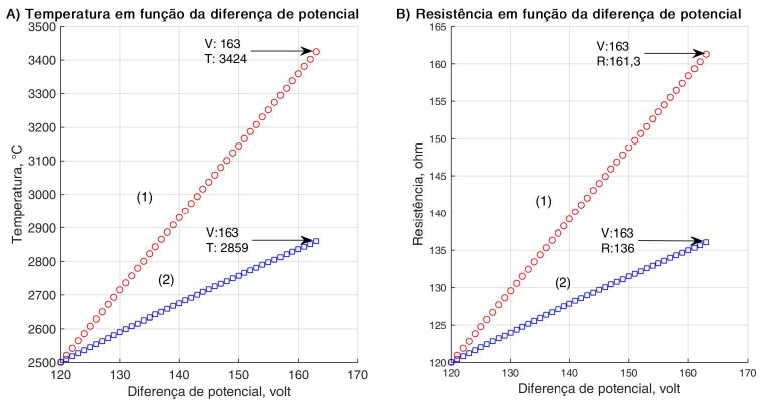
\includegraphics[scale=.99]{img-livro012018latex.jpg}
\caption{Comportamento físico do filamento.}
\label{fig:plot}
\end{figure}
\end{center}


A figura \ref{fig:plot} descreve os resultados em dois subgráficos Em (A), o conjunto de pontos $(1)$ representa a temperatura $\theta$, cujo cálculo foi baseado na 1ª hipótese e o conjunto de pontos $(2)$ representa a temperatura $\Theta$, cujo cálculo foi baseado na 2ª hipótese. As disposições dos conjuntos de pontos mostram que a temperatura do filamento aumenta à medida que a diferença de potencial aumenta de valor. Tomando em consideração que a temperatura de fusão do tungstênio é de $3422\celsius$, o conjunto de pontos $(1)$ indica que o filamento queimará por volta dos $163V$, e o conjunto de pontos $(2)$ indica que essa condição acontecerá com uma tensão superior à $163V$. A explicação para isso não está no propósito deste livos, mas uma boa sugestão seria admitir que o fluxo de energia irradiado pela lâmpada seja influenciado pela combinação das duas hipóteses.    
Em $(B)$, o conjunto de pontos $(1)$, representa a resistência $R$, cujo cálculo foi baseado na 1ª hipótese e o conjunto de pontos (2) representa a resistência $R'$, cujo cálculo foi baseado na 2ª hipótese. As disposições dos conjuntos de pontos mostram o que se presume do comportamento da resistência não-ôhmica, ou seja, se nós aplicarmos a lei de Ohm, nós encontraremos valores diferentes de resistência conforme a tensão aplicada.

\bibliographystyle{plain}
\bibliography{references}

\newpage
\appendix
\section{Algoritmo}

%%%%%%%%%%%%%%%%%%%%%%%%%%%%%%%%%%%%%%%%%%%%%%%%%%%%%%%%%%%%%%%
%Algoritmo
\begin{algorithm}[H]

\clearpage
\floatname{algorithm}{Algoritmo}
\label{alg1}
\caption{\textsc{Passo a passo}}
\begin{algorithmic}[1]

\Require $Temperatura$ $ambiente$ $em$ $\celsius$; $\alpha_m$; $\theta_{conhecido}<3422\celsius$; $R_0$; $V_0$; $P_0$; $N$ \Comment{$N$ é um número inteiro usado para auxiliar no alcance da precisão} 
%
\Ensure 
As temperaturas em $\celsius$ pela 1ª hipótese e pela 2ª hipótese
\Statex
%%%%%%%%%%%%%%% I N I C I O %%%%%%%%%%%%%%%
\hspace{-0.85cm}
\Return
\hspace{0.85cm}

\State definir constantes
\State definir e inicializar variáveis para a 1ª e 2ª hipótese
\While{$\theta' \leq 3422$} \Comment{$\theta'$ avaliar condição de parada}
\If{início}
\State calcular e definir valores inciais e incrementar contadores

\Else 
\State atualizar contadores

\State $\#$ início do laço das diferenças de potenciais

\While{$\epsilon > 0,1 {\OR} E>0,1$} \Comment{testar condição de parada}
\State \Comment{$\epsilon$ precisão para a 1ª; $E$, precisão para a 2ª hipótese hipótese}
\State incrementar contadores
\If{extrapolou N}\Comment{N quantidade de iterações previstas}
\State forçar o encerramento do programa

\EndIf
\If{$\epsilon > 0,1$}\Comment{avaliar precisão para a 1ª hipótese hipótese} 
\State calcular a taxa de irradiação aproximada
\State calcular a diferença de temperatura
\State atualizar a precisão $\epsilon$
\Comment{precisão para a 1ª hipótese} 
\State calcular temperaturas
\State calcular resistência
\State substituir coeficientes e parâmetros numéricos  

\EndIf
\Statex
\If{$E > 0,1$}\Comment{avaliar precisão para a 2ª hipótese hipótese}
\State calcular a taxa de irradiação aproximada 
\State calcular temperaturas
\State calcular a diferença de temperatura
\State calcular a precisão $E$
\State calcular resistência
\State calcular a diferença de temperatura
\State substituir coeficientes e parâmetros numéricos


\EndIf
\EndWhile
\EndIf 

\State atualizar contadores
    \State $V_{próximo}\longleftarrow V_{atual}+1$\Comment{Iterar $V$ em $1V$}
\EndWhile
\Statex
\hspace{-0.85cm}
\algorithmicPrint{}
\hspace{0.85cm}


\end{algorithmic}
\end{algorithm}



%Fim algoritmo
\newpage
\section{Código sugerido pelo autor}



\end{document}
